\chapter{Auswertung}
\label{cha:Auswertung}

\section{Energiekalibration und Bestimmung der Vollenergienachweiswahrscheinlichkeit}

Mithilfe einer Aufnahme des Gammaspektrums von Europium-152 werden die Kanäle der Apparatur kalibriert, um weitere Analysen zu ermöglichen.
Die aufgenommen Impulse pro Messkanal für diese Probe sind in \autoref{fig:Europium_channel_backgr} dargestellt.

\begin{figure}
    \centering
    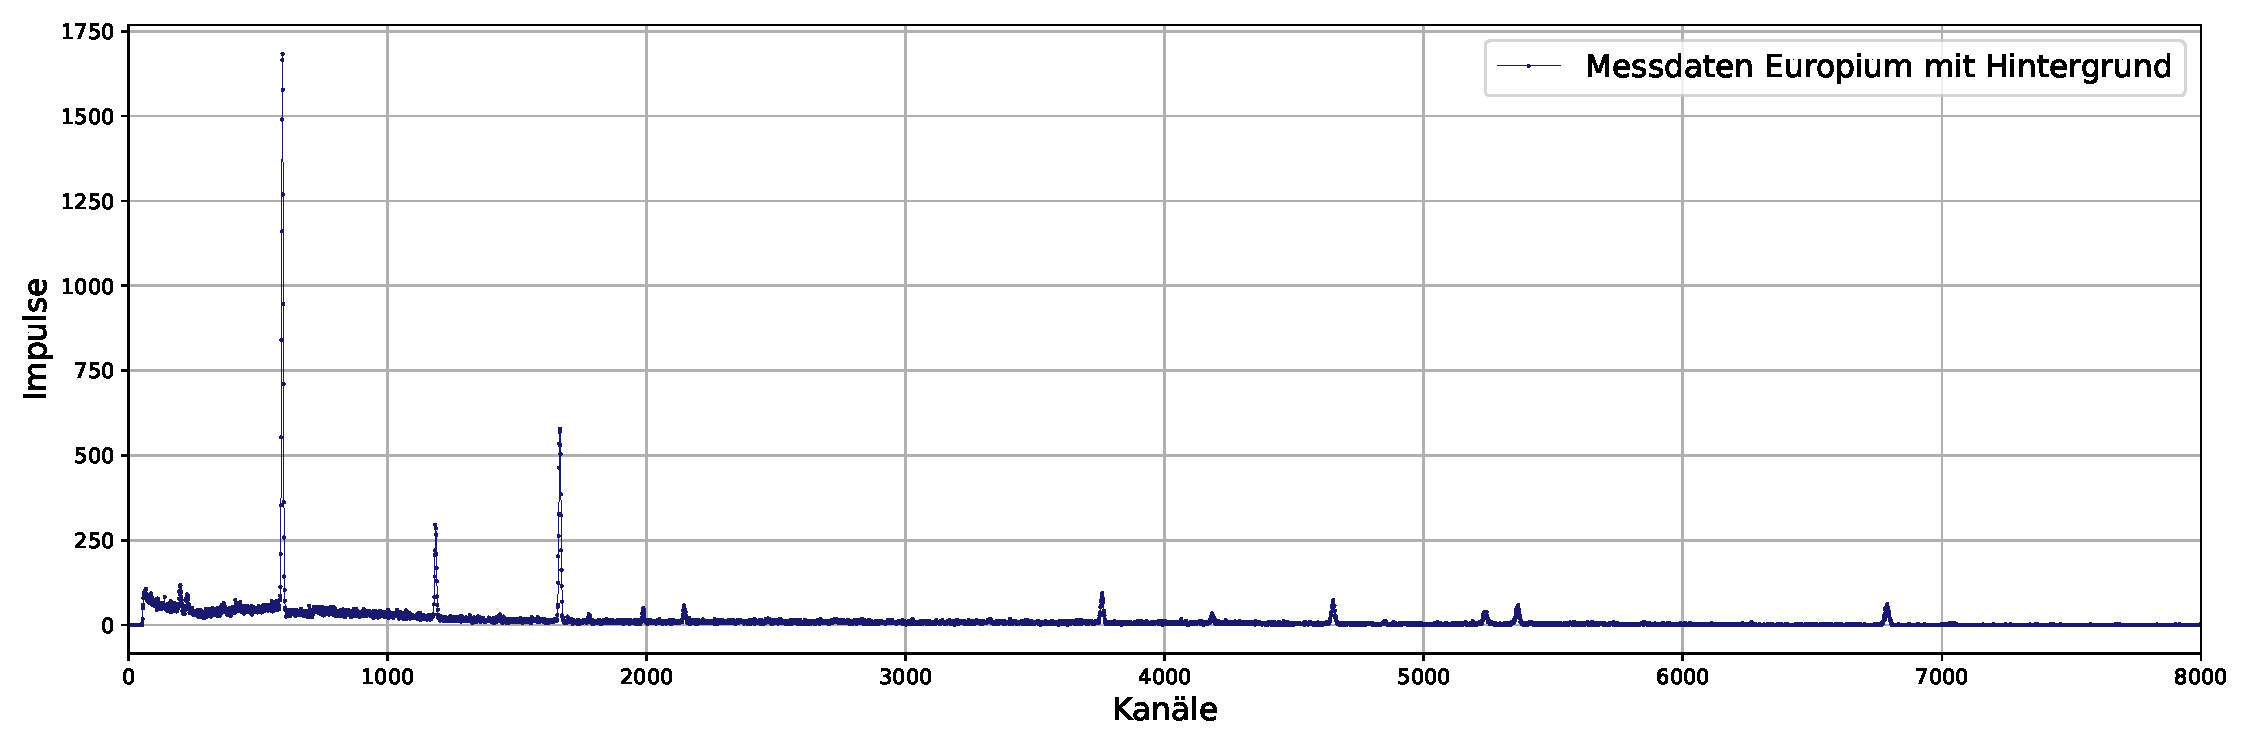
\includegraphics[width = 0.9\textwidth]{plots/europium_channel_backgr.pdf}
    \caption{Gammaspektrumaufnahme von Europium-152 in Impulsen pro Kanal. Der Hintergrund ist inkludiert.}
    \label{fig:Europium_channel_backgr}
\end{figure}

Durch Störeffekte entstehen neben den dem Material zuzuordnenden Impulsen auch jene, welche dem Hintergrund zugeordnet werden. Um diese zu identifizieren,
wird das Hintergrundspektrum des Detektors über mehrere Tage aufgenommen. Die gesamte Messzeit beträgt hier $t_{\mathrm{bg}} = \qty{71609}{\second}$. 
Diese Messung geschieht ohne eine Probe in der Apparatur. Dieses Hintergrundspektrum ist in \autoref{fig:background_channel}
dargestellt und wird jeweils von den aufgenommenen Spektren der Proben abgezogen. Das Hintergrundspektrum wird hierbei je nach Messdauer der Proben skaliert.

\begin{figure}
    \centering
    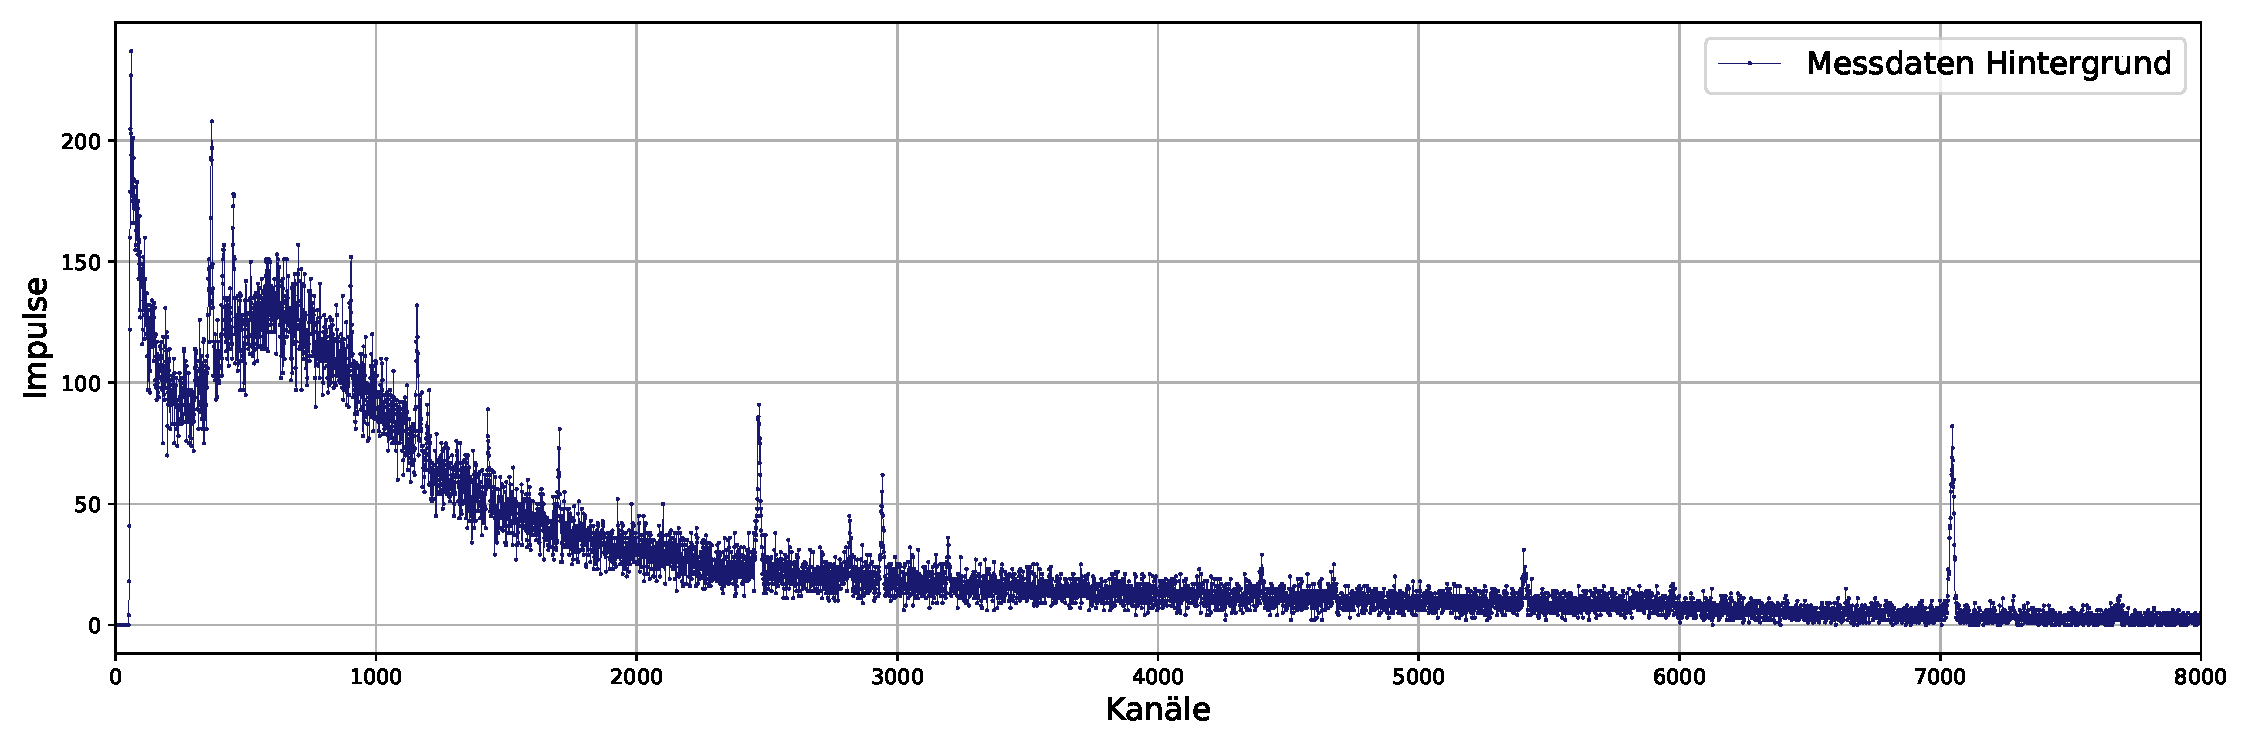
\includegraphics[width = 0.9\textwidth]{plots/background_channel.pdf}
    \caption{Gammaspektrumaufnahme des Hintergrunds in Impulsen pro Kanal.}
    \label{fig:background_channel}
\end{figure}

Das Europium-Spektrum mit Abzug des Hintergrunds ist in \autoref{fig:Europium_channel} dargestellt. Im Folgenden werden die Daten bereits um den Hintergrund bereinigt sein.

\begin{figure}
    \centering
    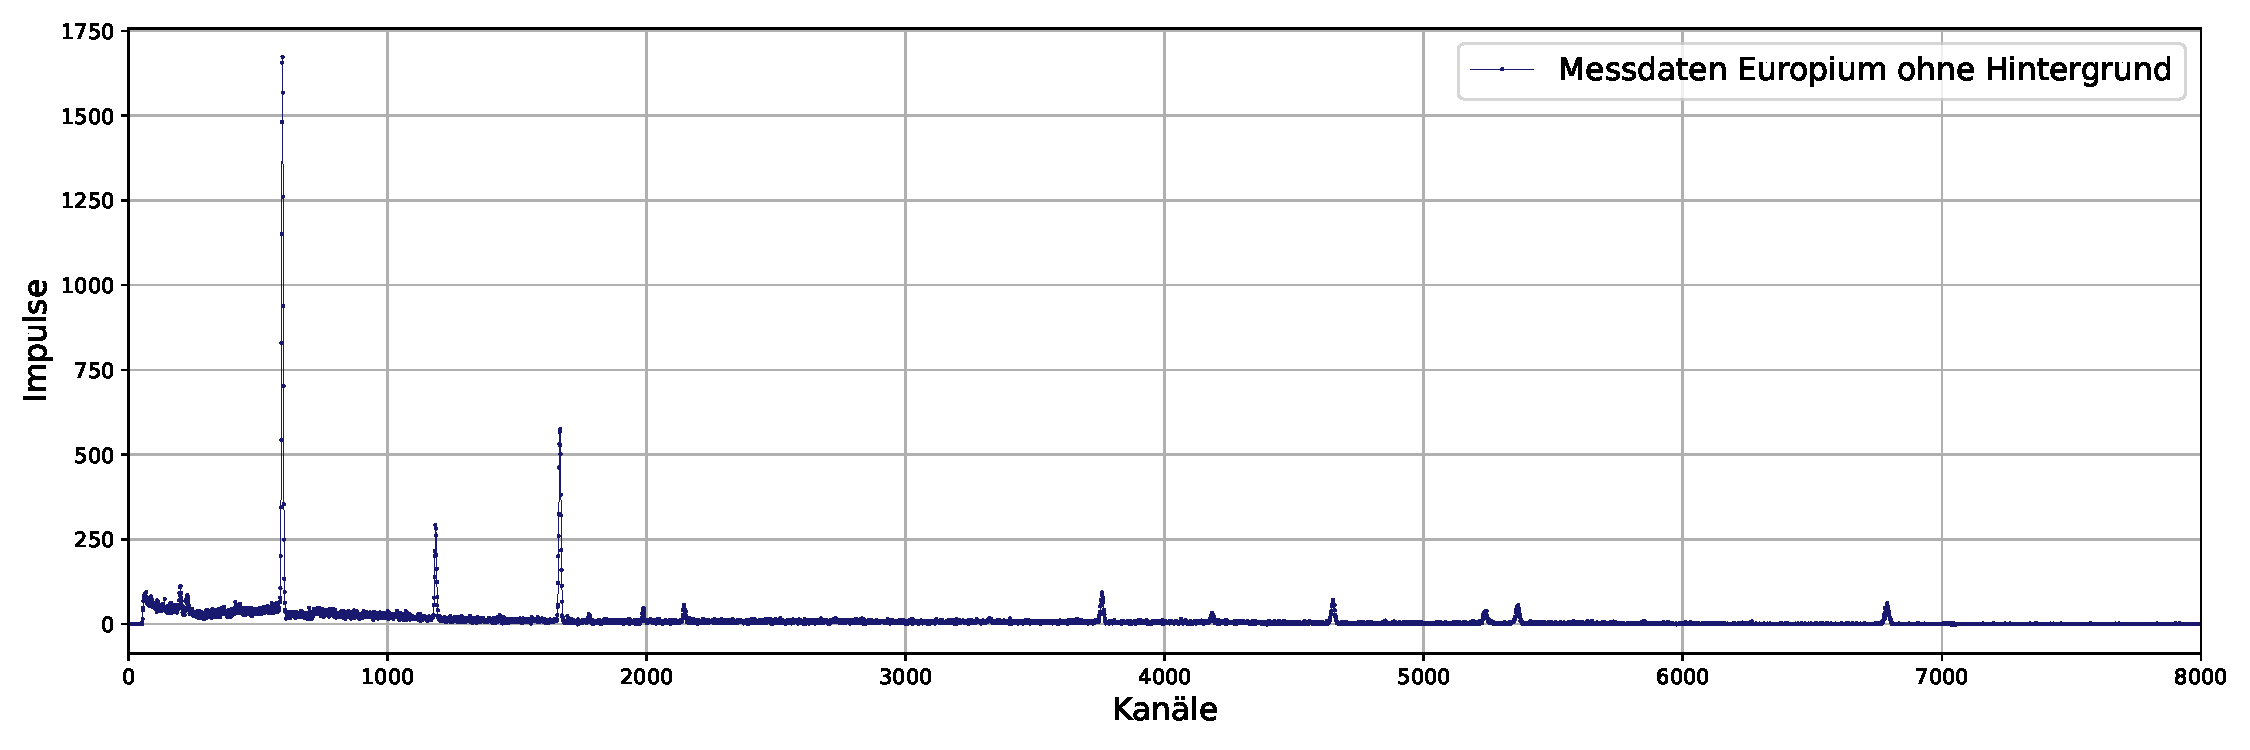
\includegraphics[width = 0.9\textwidth]{plots/europium_channel.pdf}
    \caption{Gammaspektrumaufnahme von Europium-152 in Impulsen pro Kanal. Der Hintergrund ist exkludiert.}
    \label{fig:Europium_channel}
\end{figure}

\subsection{Energiekalibration}

Für die Energiekalibration werden die für das Europium-152 spezifischen Full Energie Peaks (FEP) in dem Spektrum ausfindig gemacht und jenen aus \autoref{tab:eu152_FEP} zugeordnet. Aufgrund von Störeffekten
wird der erste signifikante Peak im Niederenergiebereich im Folgenden nicht berücksichtigt. Zudem werden nur jene FEP verwendet, welche eine Emissionswahrscheinlichkeit von über $\qty{2}{\%}$ haben.
Es lässt sich hier ein linearer Zusammehang erkennen und mithilfe der Python Bibliothek Scipy \cite{scipy} eine Ausgleichsgerade berechnen. Die Form dieser Gerade ist gegeben durch
\begin{equation}
    \mathrm{E(Kanal)} = a \cdot \mathrm{Kanal} + b.
\end{equation}
Die Parameter ergeben sich zu $a = \qty{0.2075 \pm 0.0001}{}$ und $b = \qty{-1.259 \pm 0.219}{}$, womit sich der Zusammehang zwischen Kanalnummer und Energie bestimmen lässt:
\begin{equation}
    \mathrm{E(Kanal)} = \qty{0.2075 \pm 0.0001}{} \cdot \mathrm{Kanal} + \qty{-1.259 \pm 0.219}{}.
\end{equation}
Die berechnete Gerade mitsamt Messwerte ist in \autoref{fig:Energie_Kanal} zu sehen.

\begin{figure}
    \centering
    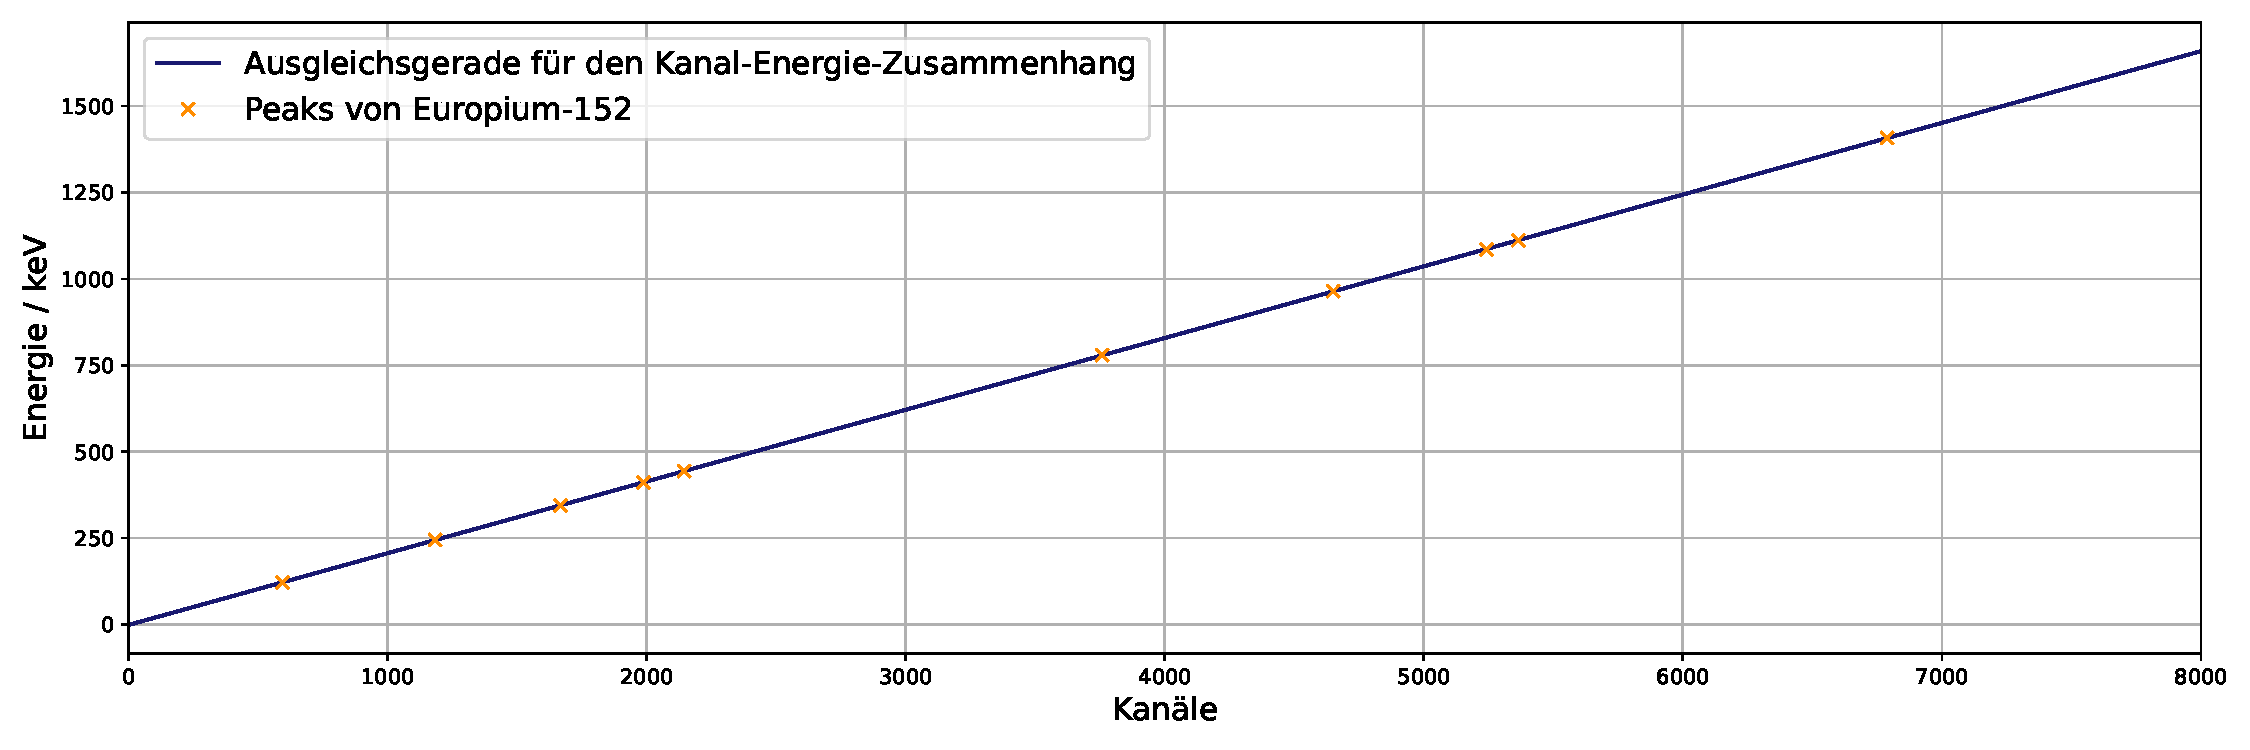
\includegraphics[width = 0.8\textwidth]{plots/energy_channel.pdf}
    \caption{Linearer Zusammehang des Detektors zwischen der Kanalnummer und Energie.}
    \label{fig:Energie_Kanal}
\end{figure}

\subsection{Vollenergienachweiswahrscheinlichkeit}

Um die Vollenergienachweiswahrscheinlichkeit zu bestimmen, wird der Zusammenhang
\begin{equation}
    \label{eqn:quality}
    Q = \frac{Z 4 \pi}{AWt \Omega}
\end{equation}
verwendet. $Z$ ist hier der Linieninhalt des FEPs, $W$ dessen Emissionswahrscheinlichkeit, $A$ die Aktivität der Probe am Tag der Messung (06.11.2023), $t$ die
Messdauer und $Omega$ der durch den Detektor abgedeckten Raumwinkel.\\
Der Linieninhalt der einzelnen Peaks wird über einen Fit an eine Normalverteilung mittels Scipy\cite{scipy} und dessen Integration bestimmt. Die Linieninhalte, sowie die Emissionswahrscheinlichkeiten sind in \autoref{tab:eu152} zu finden.
Die Aktivität der Probe lässt sich über das Zerfallsgesetz
\begin{equation}
    A(t) = A_0 \exp{(-\frac{\ln{(2)}}{\tau}t)}
\end{equation}
bestimmen, wobei $A_0$ die Aktivität an einem bestimmten Tag ist und $t$ die seit diesem Tag verstrichene Zeit. $\tau$ ist die Halbwertszeit von Europium-152 und ist gegeben 
durch $\tau_{\mathrm{Eu}} = \qty{13.54}{\mathrm{a}} = \qty{426902400}{\second}$\cite{Gammaspektrum_Eu152}. Die Europium-152-Probe hatte am 01.10.2000 eine Aktivität von $A_0 = \qty{4130 \pm 60}{\becquerel}$\cite{v18}. Seit 
diesem Tag sind $t=\qty{728524800}{\second}$ vergangen. Somit ergibt sich eine Aktivität des Europium-152 von 
\begin{equation}
    A_{Eu} = \qty{1265 \pm 18}{\becquerel}
\end{equation}
für den Messtag.\\
Der abgedeckte Raumwinkel lässt sich durch eine Kleinwinkelnäherung des Sinus als
\begin{equation}
    \Omega = \frac{4\pi}{2}(1-\frac{a}{\sqrt{a^2+r^2}})
\end{equation}
annähern. Hierbei ist $a = \qty{8.51 \pm 0.005}{\centi\metre}$ der Abstand zwischen der Europium-Probe und der Aluminiumabdeckung des Detektors und $r=\qty{2.25}{\centi\metre}$\cite{v18} der Radius
der Auftrefffläche des zylinderförmigen Detektors. Die Vollenergienachweiswahrscheinlichkeit lässt sich nun für jeden Peak berechnen. Eine Ausnahme bildet der erste FEP, da aufgrund der Störeffekte nur Energien,
 welche größer als $\qty{150}{\kilo\electronvolt}$ berücksichtigt werden. Mithilfe von Scipy\cite{scipy} wird nun der Potenzansatz
\begin{equation}
    Q(E) = a(E)^b \frac{1}{\qty{}{\kilo\electronvolt}}
\end{equation}
an die Messwerte gefittet. Die resultierende Funktion ist in \autoref{fig:quality} zu finden, sowie die einzelnen Messwerte in \autoref{tab:eu152}. Die Parameter der Regression lauten
\begin{align}
    \label{Q_params}
    a &= \qty{110.6 \pm 41.3}{},\\
    b &= \qty{-1.053 \pm 0.064}{}.
\end{align}
Somit ergibt sich folgender Zusammenhang zwischen dem Vollenergienachweiswahrscheinlichkeit und der Energie:
\begin{equation}
    Q(E) = \qty{110.6 \pm 41.3}{}\cdot E^{\qty{-1.053 \pm 0.064}{}} \qty{}{\per\kilo\electronvolt}.
\end{equation}
\begin{figure}
    \centering
    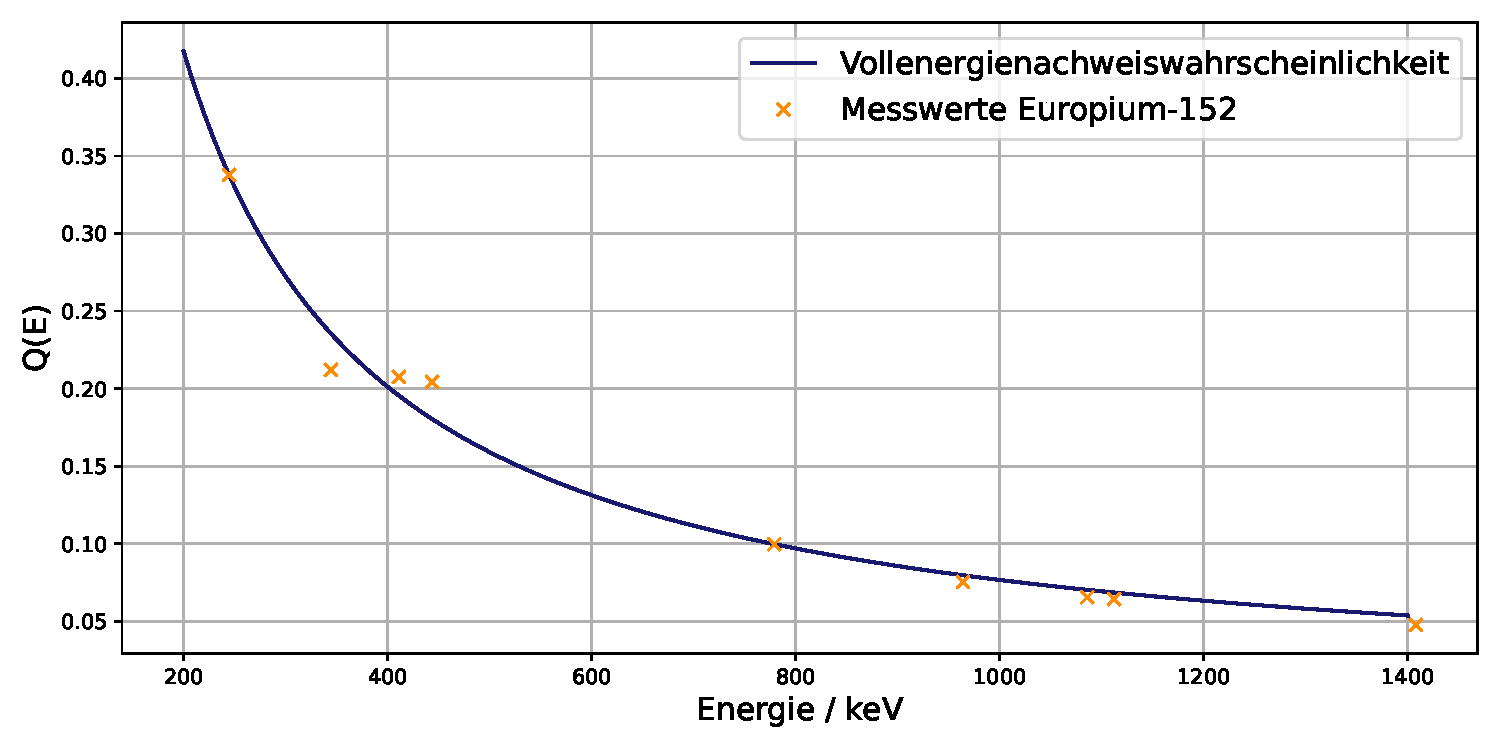
\includegraphics[width = 0.8\textwidth]{plots/quality.pdf}
    \caption{Die Vollenergienachweiswahrscheinlichkeit des Detektors in Abhängigkeit von der Energie.}
    \label{fig:quality}
\end{figure}

\begin{table}
    \centering
    \caption{Linieninhalt $Z$, Emissionswahrscheinlichkeit $W$ und Vollenergienachweiswahrscheinlichkeit $Q$ pro FEP für Europium-152.}
    \label{tab:eu152}
    \begin{tabular}{c c c c}
      \toprule
      $Z \mathbin{/} \mathrm{Impulse}$ & $W \mathbin{/} \% $ & $E_{\mathrm{FEP}} \mathbin{/} \unit{\kilo\electronvolt}$ & $Q \mathbin{/} \%$ \\
      \midrule
      $\qty{2509}{} $ & $\qty{7.6}{}$ & $244.7$ & $\qty{33.79 \pm 0.49}{}$ \\
      $\qty{5491}{}$ & $\qty{26.5}{}$ & $344.3$ & $\qty{21.21 \pm 0.31}{}$ \\
      $\qty{446}{}$ & $\qty{2.2}{}$ & $411.12$ & $\qty{20.77 \pm 0.30}{}$ \\
      $\qty{618}{}$ & $\qty{3.1}{}$ & $443.96$ & $\qty{20.43 \pm 0.29}{}$ \\
      $\qty{1256}{}$ & $\qty{12.9}{}$ & $778.9$ & $\qty{9.96 \pm 0.15}{}$ \\
      $\qty{1079}{}$ & $\qty{14.6}{}$ & $964.08$ & $\qty{7.56 \pm 0.11}{}$ \\
      $\qty{654}{}$ & $\qty{10.2}{}$ & $1085.9$ & $\qty{6.56 \pm 0.09}{}$ \\
      $\qty{855}{}$ & $\qty{13.6}{}$ & $1112.1$ & $\qty{6.43 \pm 0.09}{}$ \\
      $\qty{979}{}$ & $\qty{21.0}{}$ & $1408.0$ & $\qty{4.77 \pm 0.07}{}$ \\
      \bottomrule
    \end{tabular}
\end{table}

\section{Monochromatisches Gammaspektrum eines Caesium-137-Strahlers}

In diesem Abschnitt wird das monochromatische Gammaspektrum einer Caesium-137-Probe untersucht. Hierfür werden, wie auch für das Europium-Spektrum, das 
Hintergrundspektrum abgezogen. Das reine Caesium-Gammaspektrum ist in \autoref{fig:caesium} dargestellt.
\begin{figure}
    \centering
    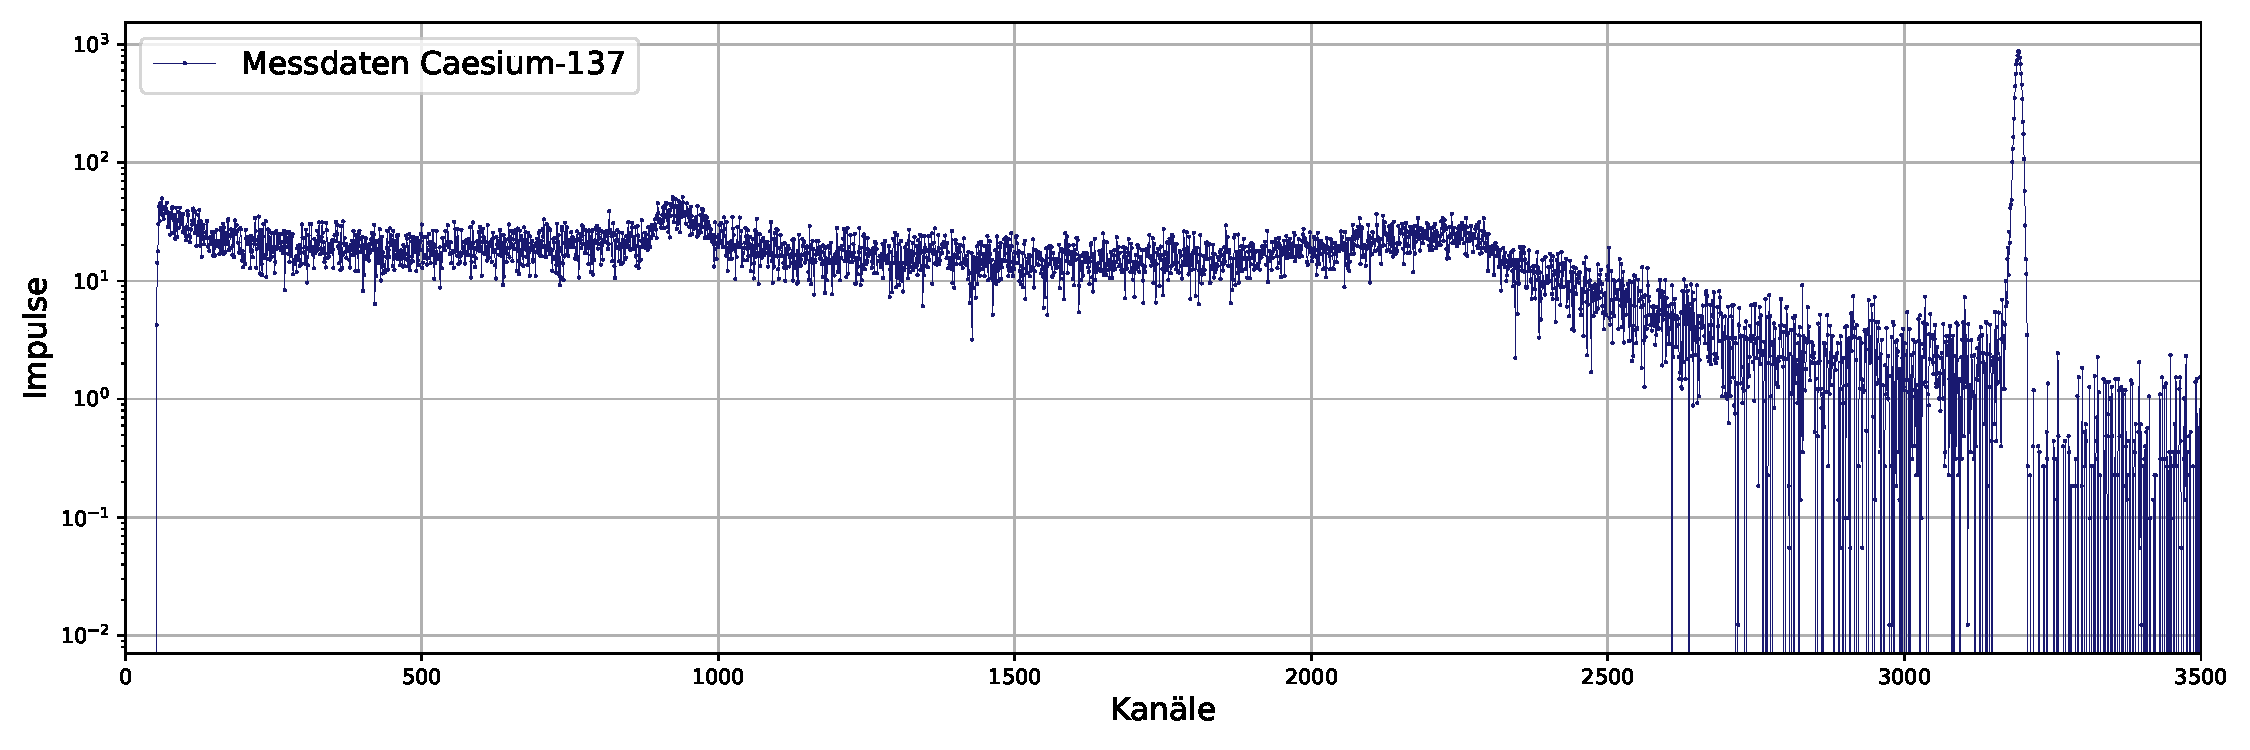
\includegraphics[width = 0.8\textwidth]{plots/caesium_channel.pdf}
    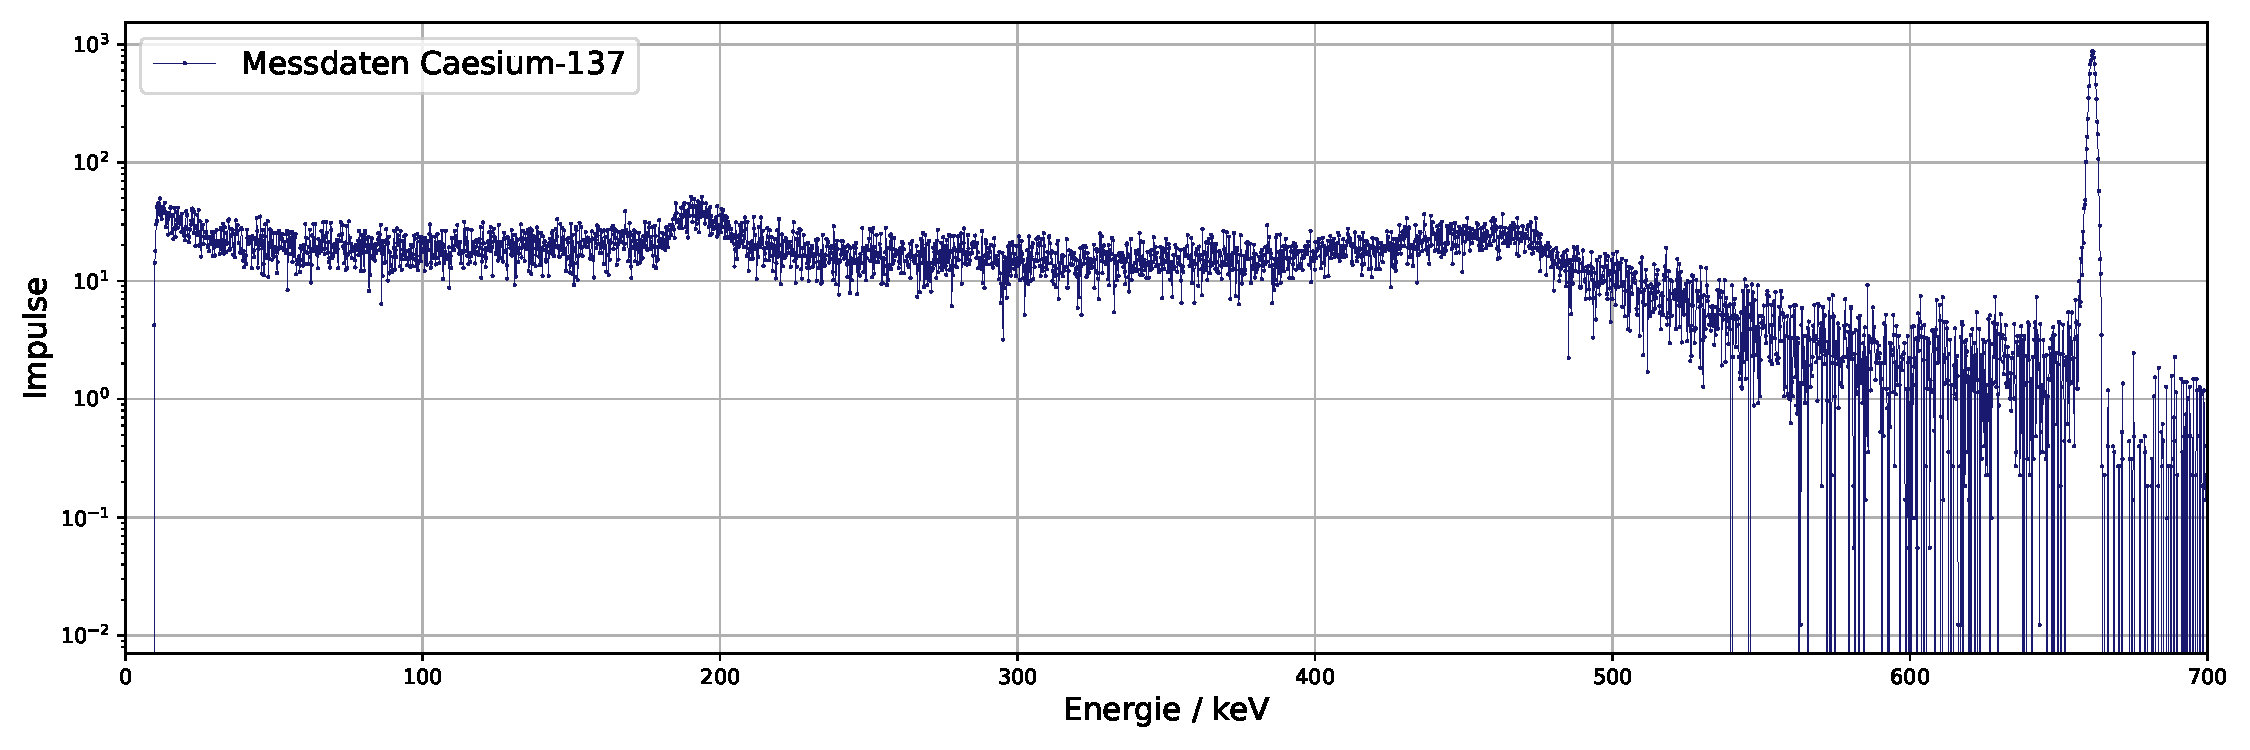
\includegraphics[width = 0.8\textwidth]{plots/caesium_energy.pdf}
    \caption{Gammaspektrumaufnahme des Caesium-137-Strahlers pro Kanal (oben) und pro Energie in keV (unten). Die Kanäle (bzw. Energie) wurden auf den relevanten Bereich reduziert.}
    \label{fig:caesium}
\end{figure}
Es wird zunächst der FEP bei circa $E_{\gamma} = \qty{661.66}{\kilo\electronvolt}$ untersucht. Hierfür wird eine Normalverteilung an die Messwerte mithilfe von Scipy\cite{scipy} gefittet und die Parameter bestimmt.
Die Normalverteilung ist gegeben durch
\begin{equation}
    f_{\mathrm{Norm}}(x) = \frac{a}{\sqrt{2\pi}\sigma^2}\exp{(-\frac{(x-\mu)^2}{2\sigma^2})}.
\end{equation}
Der Mittelwert der Verteilung ist $\mu$, die Stadardabweichung ist $\sigma$, $a$ ist ein Vorfaktor und $x$ beschreibt hier die Kanäle. Die Parameter
bestimmen sich zu
\begin{align}
    a &= \qty{10370 \pm 40}{},\\
    \mu &= \qty{3193 \pm 0}{},\\
    \sigma &= \qty{4.740 \pm 0.019}{}.
\end{align}
Die Halbwerts- und Zehntelwertsbreite wird mithilfe der Messdaten bestimmt. Die Halbwerts- bzw. Zehntelwertsbreite
bestimmt sich hierbei über die Breite der Verteilung, bei der Hälfte bzw. dem Zehntel des Maximums. Das Maximum und die Höhe der Halbwerts-/Zehntelwertsbreite der Normalverteilung bestimmt sich zu
\begin{align}
    \mathrm{Max}_{\mathrm{norm}}    &= \qty{873 \pm 5}{},\\
    I_{\mathrm{Halb, norm}}         &= \qty{436.3 \pm 2.3}{},\\
    I_{\mathrm{Zehntel, norm}}      &= \qty{87.3 \pm 0.5}{}.
\end{align}
Bei Normalverteilungen herrscht zwischen diesen zwei Kenngrößen folgende konstante Beziehung:
\begin{equation}
    \frac{E_{\mathrm{FWTM, norm}}}{E_{\mathrm{FWHM, norm}}} = \qty{1.822615}{}.
\end{equation}
Da die Messwerte einer Normalverteilung folgen sollen, sollte dieser Zusammenhang auch für die Messwerte gelten. Die Halbwerts- und Zehntelwertsbreite der Messwerte ergibt sich zu 
\begin{align}
    E_{\mathrm{FWHM}}    &= \qty{2.316 \pm 0.009}{},\\
    E_{\mathrm{FWTM}}     &= \qty{4.222 \pm 0.017}{}.
\end{align}
Für den Quotienten ergibt sich somit:
\begin{equation}
    \frac{E_{\mathrm{FWTM, exp}}}{E_{\mathrm{FWHM, exp}}} = \qty{1.822616}{}.
\end{equation}
Der FEP des Caesium-137, sowie Halbwerts- und Zehntelwertsbreite sind in \autoref{fig:Cs_FEP} zu finden.\\
\begin{figure}
    \centering
    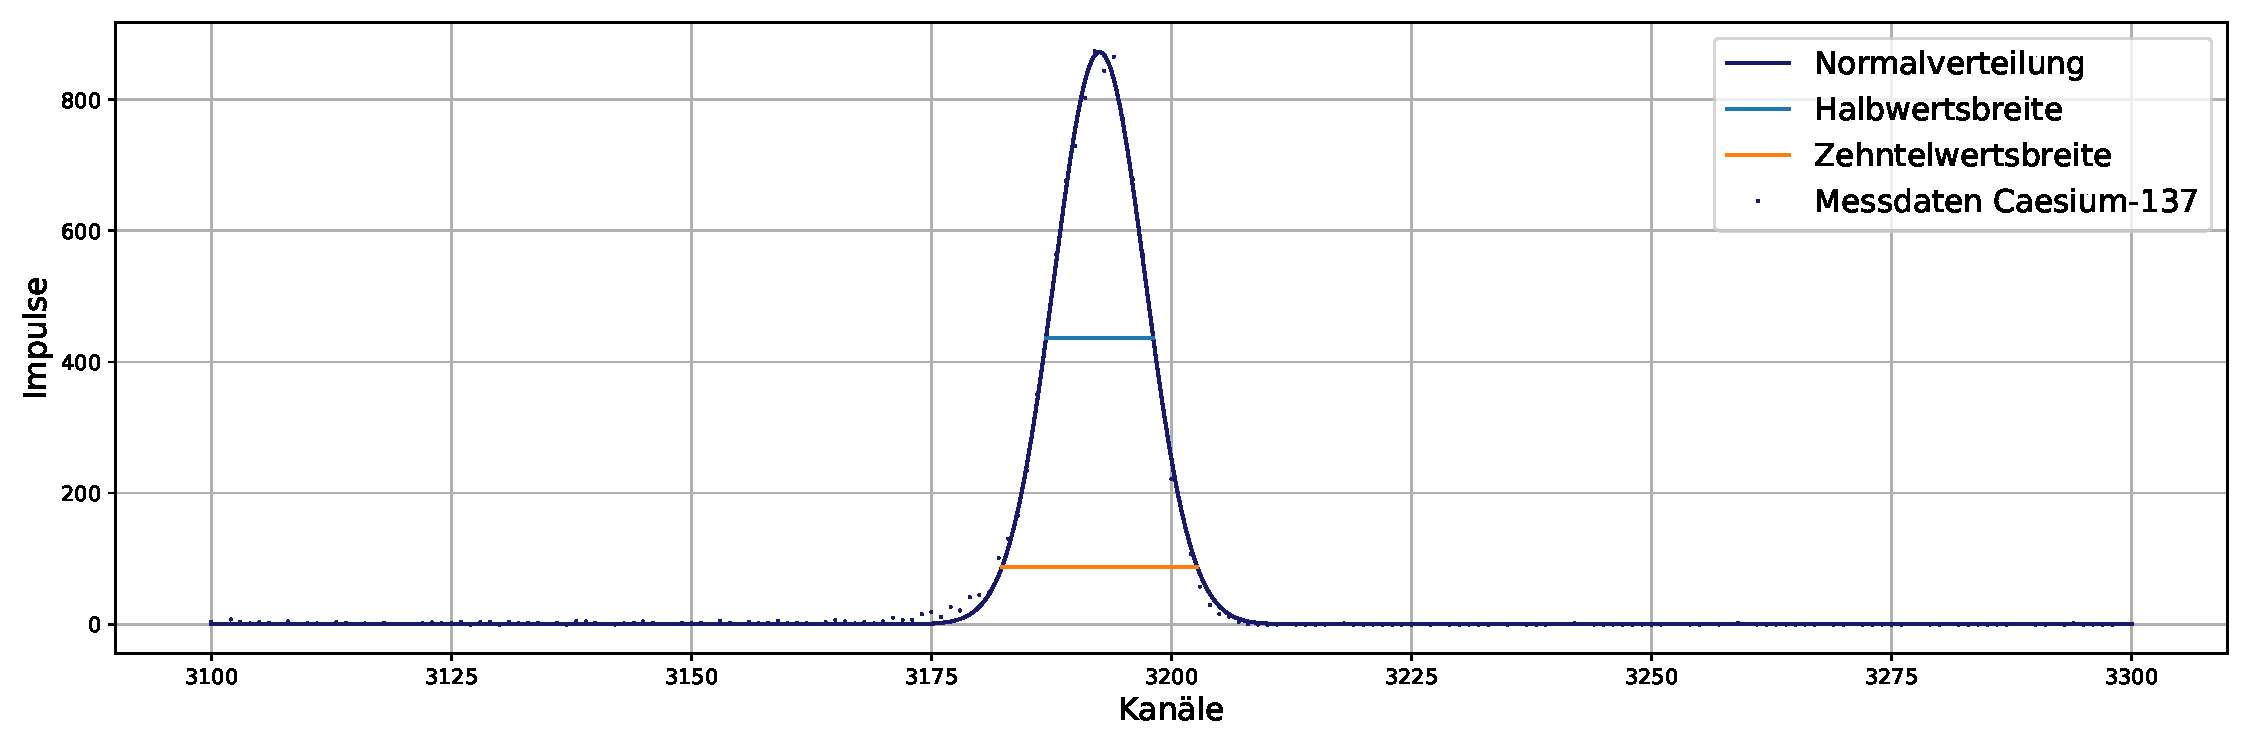
\includegraphics[width = 0.8\textwidth]{plots/caesium_channel_gauss_fit.pdf}
    \caption{FEP des Caesium-137 mitsamt Halbwerts- sowie Zehntelwertsbreite und Normalverteilung nach Kanal.}
    \label{fig:Cs_FEP}
\end{figure}
Durch Integration über die Normalverteilung lässt sich außerdem der Inhalt des FEP zu $Z_{\mathrm{Cs, FEP}} = \qty{10366}{\mathrm{Impulse}}$ bestimmen.\\
Um den Inhalt des Compton-Kontinuums zu bestimmen, muss diese zunächst an eine Funktion gefittet werden. Da der untere Energiebereich durch
viele Störfaktoren geprägt ist, wird lediglich der Breich zwischen $\qty{250}{\kilo\electronvolt}$ und $\qty{470}{\kilo\electronvolt}$ für
das fitten verwendet. \\
Als Basis für den Funktionsansatz wird \autoref{eqn:WQ_compton} verwendet. Diese Gleichung wird durch einen konstanten Vorfaktor erweitert, welcher
sich mithilfe von Scipy\cite{scipy} als
\begin{equation}
    a = \qty{9.205 \pm 0.080}{}
\end{equation}
ergibt. Dieser Faktor beinhaltet alle konstanten Vorfaktoren von \autoref{eqn:WQ_compton}. Eine Integration über das Compton-Kontinuum ergibt schließlich
\begin{equation}
    Z_{\mathrm{Cs, C}} = \qty{36543}{\mathrm{Impulse}}.
\end{equation}
Somit haben der FEP und das Compton-Kontinuum ein Verhältnis von $\frac{Z_{\mathrm{Cs, C}}}{Z_{\mathrm{Cs, FEP}}} = \qty{3.53}{}$. Das Compton-Kontinuum mitsamt Regression sind in \autoref{fig:Cs_Compton} gezeigt.
\begin{figure}
    \centering
    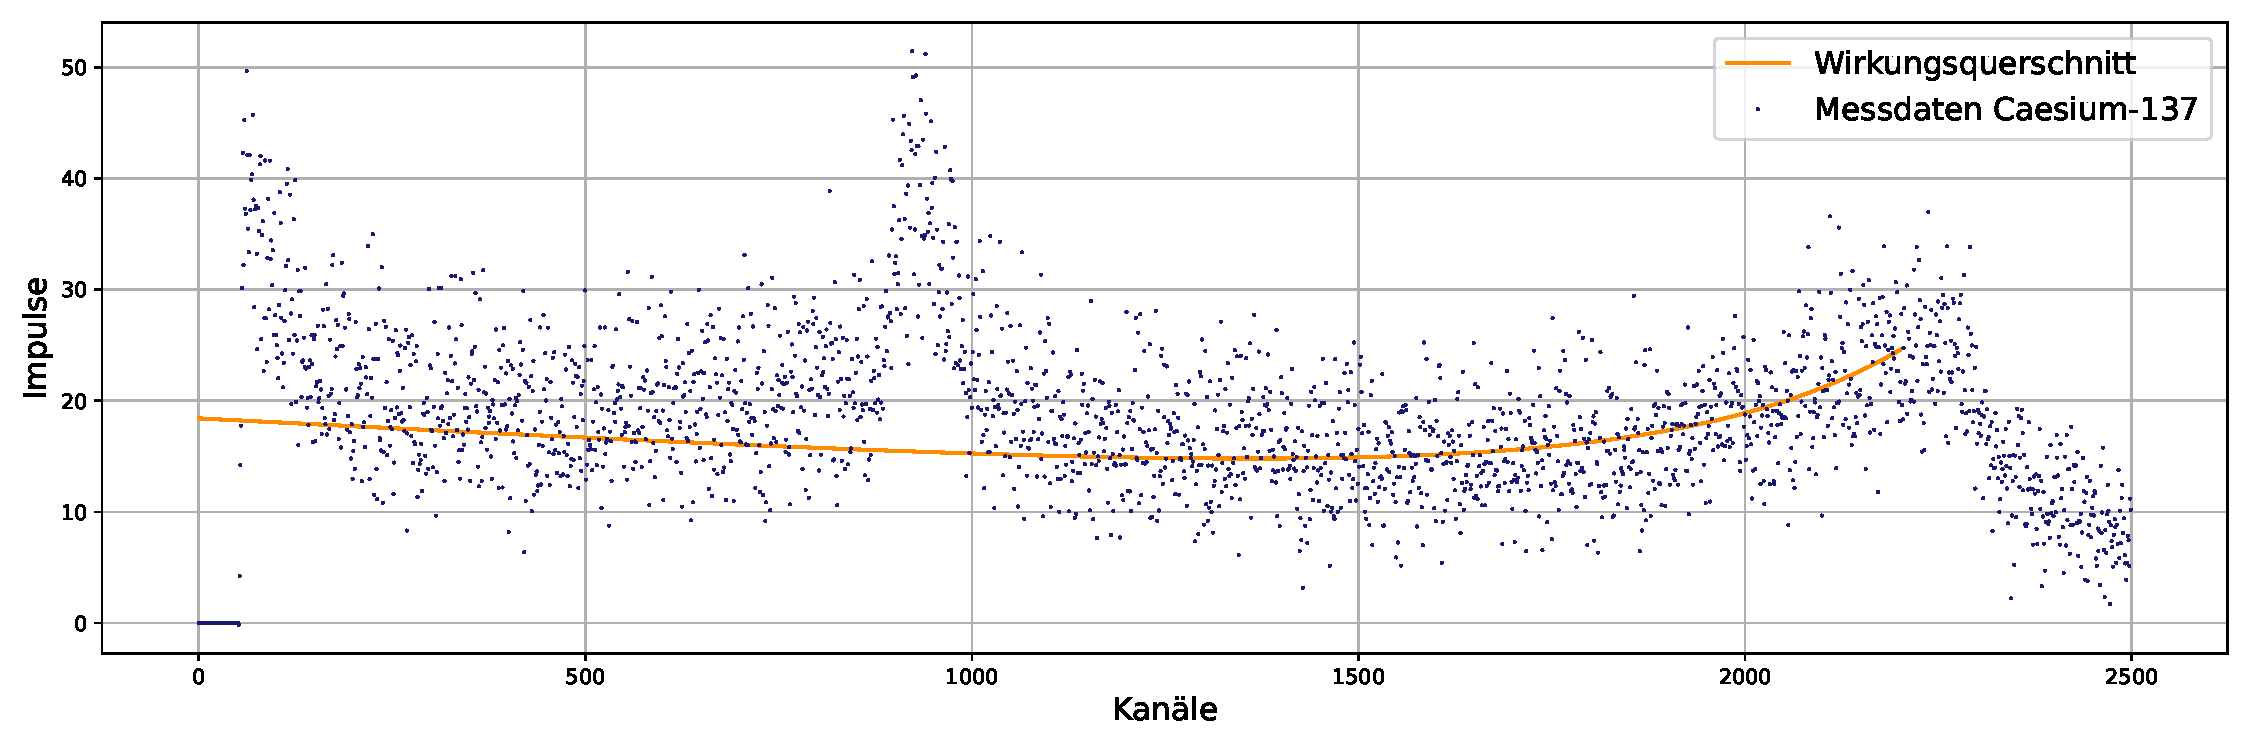
\includegraphics[width = 0.8\textwidth]{plots/caesium_compton_channel.pdf}
    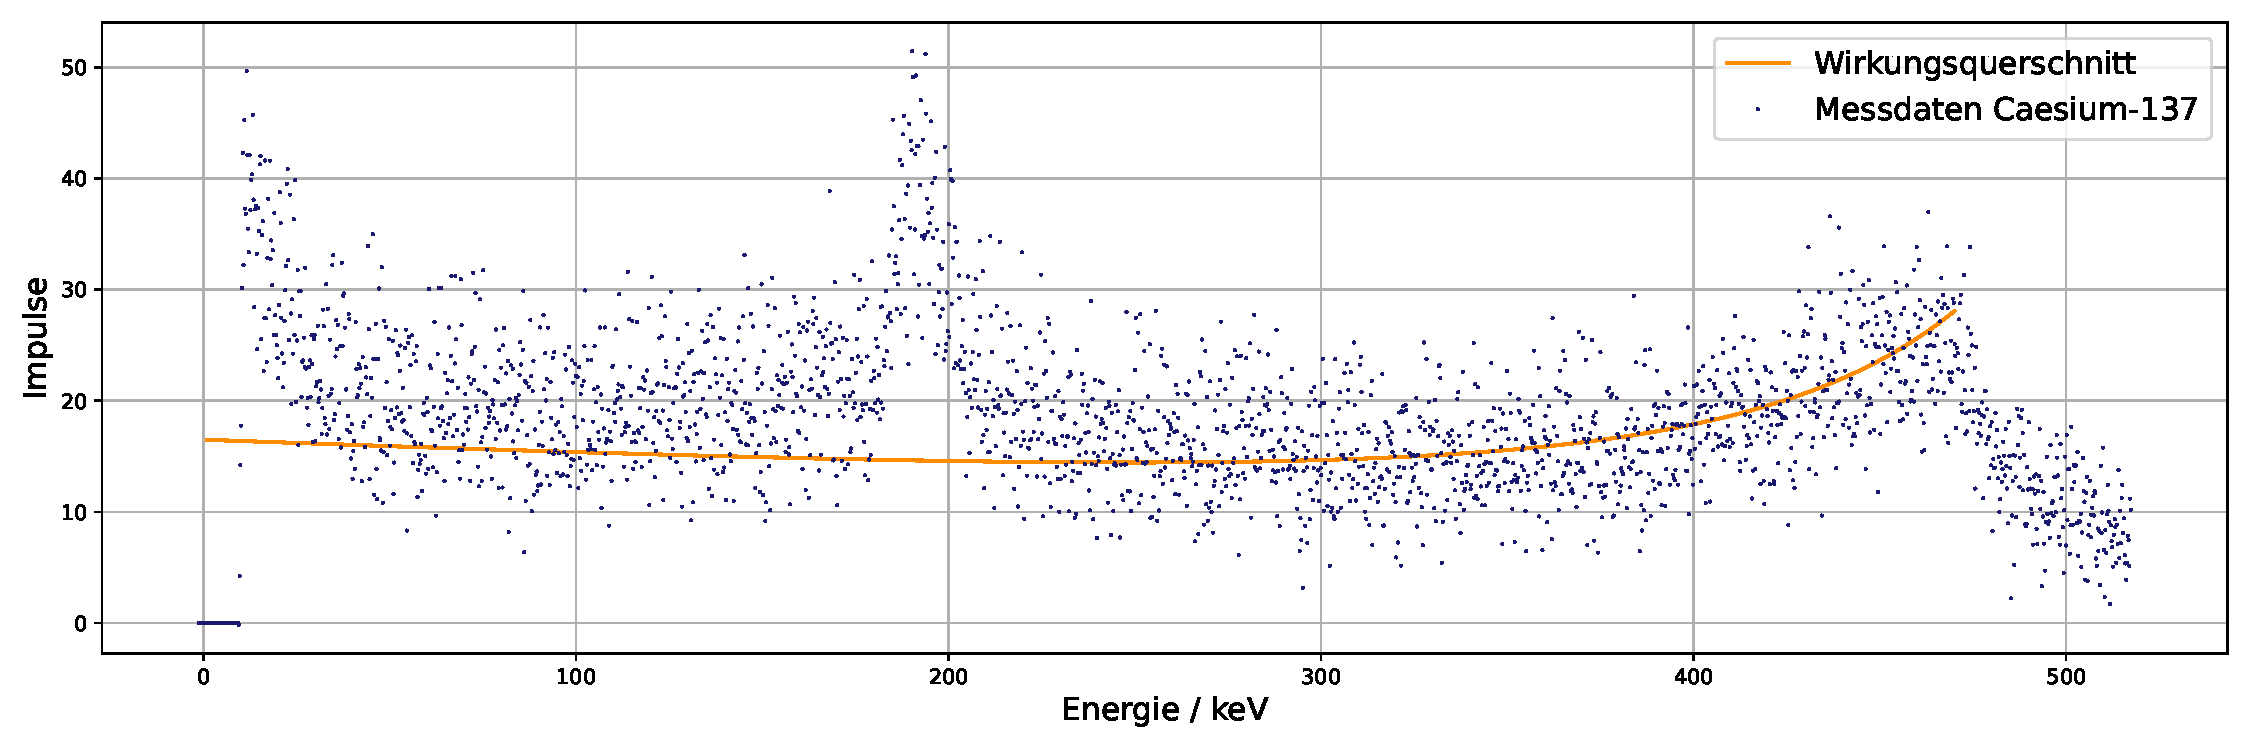
\includegraphics[width = 0.8\textwidth]{plots/caesium_compton_energy.pdf}
    \caption{Compton-Kontinuum des Caesium-137 und Compton-Wirkungsquerschnitt pro Kanal (oben) und pro Energie in keV (unten). Die Kanäle (bzw. Energie) wurden auf den relevanten Bereich reduziert.}
    \label{fig:Cs_Compton}
\end{figure}
Über \autoref{fig:Cs_Compton} lassen sich die Position der Compton-Kante $E(\mathrm{CK})$ und des Rückstreupeaks $E(\mathrm{RS})$ ablesen. Es wird ein Ablesefehler von $\qty{1}{\kilo\electronvolt}$
berücksichtigt:
\begin{align}
    E_{\mathrm{exp}}(\mathrm{CK}) &= \qty{470 \pm 1}{\kilo\electronvolt},\\
    E_{\mathrm{exp}}(\mathrm{RS}) &= \qty{190 \pm 1}{\kilo\electronvolt}.
\end{align}
Hierzu lassen sich die theoretischen Erwartungswerte berechnen. Die Energie des Gammaquant beträgt $E_{\gamma} = \qty{661.66}{\kilo\electronvolt}$. Für die Position des
Rückstreupeaks wird \autoref{eqn:Rückstreupeak} verwendet und $E_{\gamma}$ eingesetzt. $\epsilon$ ist hier das Verhältnis der Energie des Gammaquants zu der Ruheenergie des
Elektrons. Für die Compton-Kante wird \autoref{eqn:comptonkante} herangezogen. Somit ergibt sich für die theoretischen Werte 
\begin{align}
    E_{\mathrm{th}}(\mathrm{CK}) &= \qty{477.34}{\kilo\electronvolt},\\
    E_{\mathrm{th}}(\mathrm{RS}) &= \qty{184.32}{\kilo\electronvolt}.    
\end{align}
Um die Absorptionswahrscheinlichkeit zu berechnen, wird
\begin{equation}
    \label{eqn:Prob}
    P(l) = 1-\exp{(-\mu l)}
\end{equation}
verwendet, wobei $\mu$ der Extinktionskoeffizient ist, ablesbar in \autoref{fig:germanium_wq} und $l$ die im Detektor zurückgelegte Strecke. Die Detektorlänge beträgt $l = \qty{3.9}{\centi\metre}$
und die Extinktionskoeffizienten für $E_{\gamma} = \qty{661.66}{\kilo\electronvolt}$ sind 
\begin{align}
    \mu_{\mathrm{C}} &= \qty{0.36 \pm 0.01}{\per\centi\metre},\\
    \mu_{\mathrm{Ph}} &= \qty{0.0075 \pm 0.001}{\per\centi\metre},\\
    \mu_{\mathrm{Paar}} &= \qty{0 \pm 0}{\per\centi\metre}.
\end{align}
Der Ablesefehler wird hierbei anhand der logarthmischen Skala angepasst. Der Extinktionskoeffizient für die Paarbildung beträgt $\mu_{\mathrm{Paar}} = \qty{0 \pm 0}{\per\centi\metre}$, 
da bei diesem Energiebereich keine Paarbildung auftreten kann. Eingesetzt in \autoref{eqn:Prob} ergibt sich:
\begin{align}
    P_{\mathrm{C}} &= \qty{75.4}{\%},\\
    P_{\mathrm{Ph}} &= \qty{2.9}{\%},\\
    P_{\mathrm{Paar}} &= \qty{0}{\%}.
\end{align}
Da die Absorptionswahrscheinlichkeit des Photoeffekts 26-Mal geringer ist als die des Compton-Effekts, sollte der Linieninhalt des Photopeaks dementsprechend geringer sein.

\section{Aktivitätsbestimmung von Barium-133}

Um die Aktivität einer Probe zu bestimmen, kann \autoref{eqn:quality} nach der Aktivität $A$ umgeformt werden:
\begin{equation}
    \label{eqn:Aktivitaet}
    A = \frac{Z 4 \pi}{ Q W t \Omega}.
\end{equation}
Mithilfe der bestimmten Parameter für Q (\ref{Q_params}) wird die Aktivität
für jeden signifikanten Peak berechnet und mithilfe von der Pyhton Bibliothek Uncertainties\cite{uncertainties} der Mittelwert, sowie Standardabweichung berechnet.\\
In diesem Experiment soll dies für Barium-133 unterucht werden. Das aufgenommene Spektrum abzüglich des Hintergrunds ist in \autoref{fig:Barium} zu sehen.
\begin{figure}
    \centering
    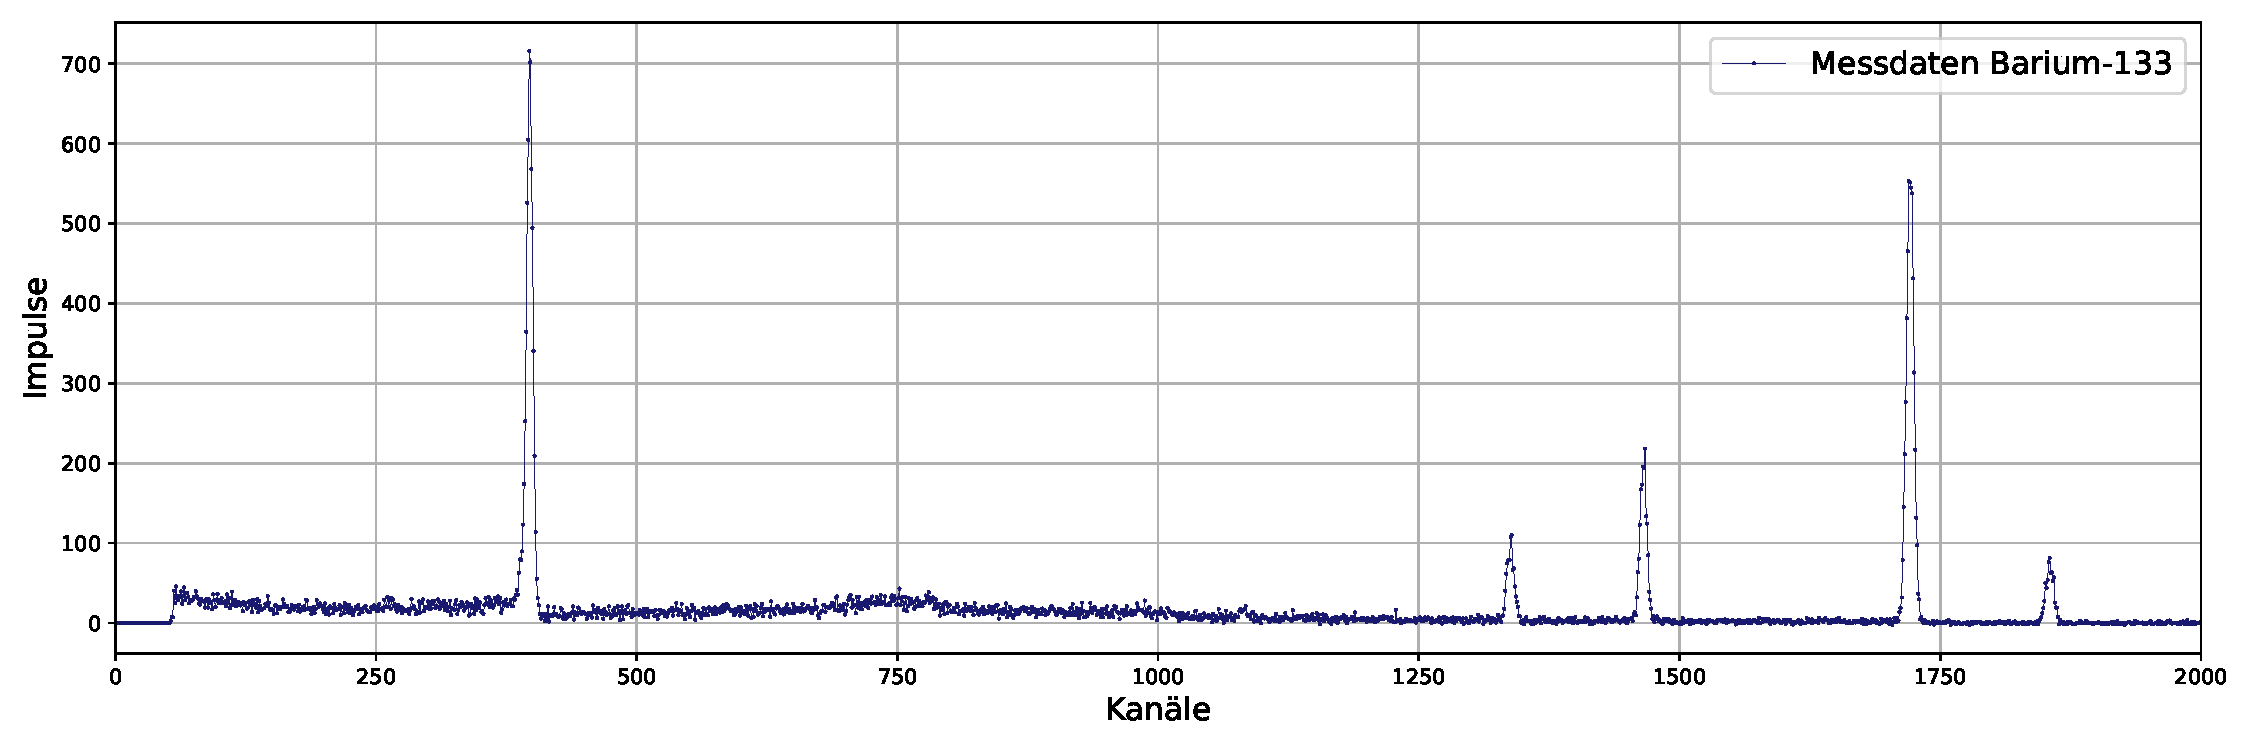
\includegraphics[width = 0.8\textwidth]{plots/barium_channel.pdf}
    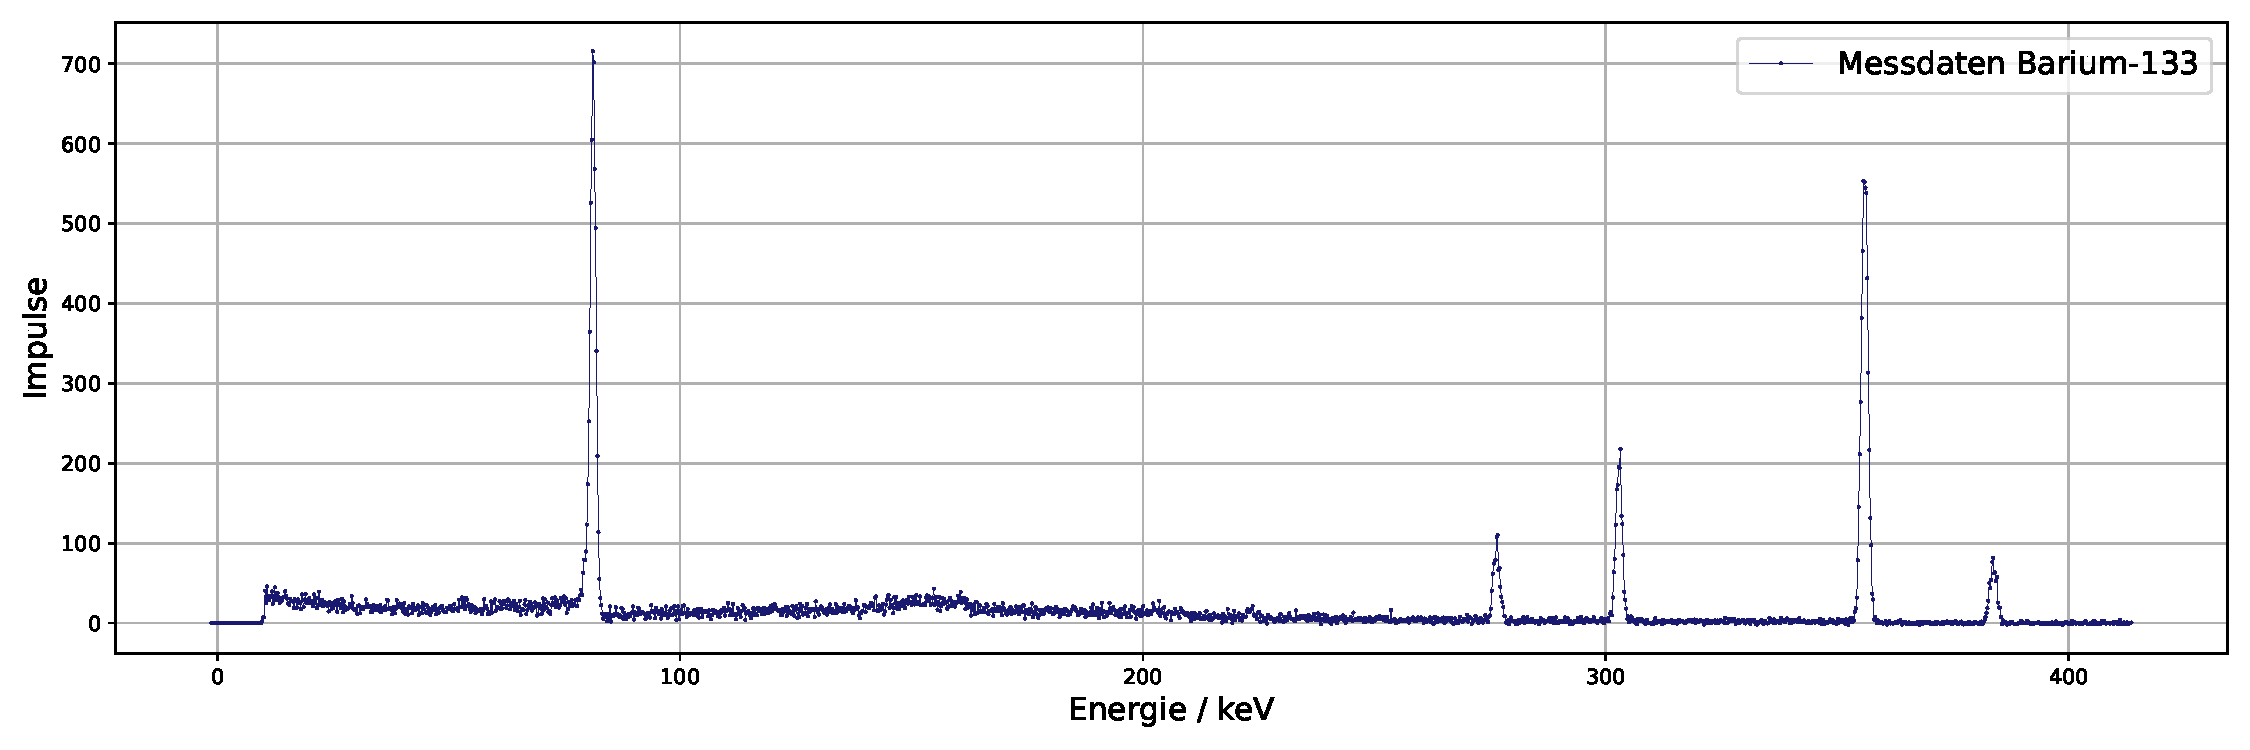
\includegraphics[width = 0.8\textwidth]{plots/barium_energy.pdf}
    \caption{Gammaspektrumaufnahme des Barium-133-Strahlers pro Kanal (oben) und pro Energie in keV (unten). Die Kanäle (bzw. Energie) wurden auf den relevanten Bereich reduziert.}
    \label{fig:Barium}
\end{figure}
Für jeden Peak wird mittels einer durch Scipy\cite{scipy} gefitteten Gaussfunktion der Linieninhalt und die Position des FEP bestimmt. Die Messdauer für Barium-133 beträgt
$t_{\mathrm{Ba}} = \qty{2876}{\second}$. Mit diesen Informationen wird schließlich die Aktivität bestimmt.\\
All diese Daten sind in \autoref{tab:Barium} aufgelistet. Bei der Berechnung wurde der erste Peak aufgrund der Störeffekte in diesem Bereich nicht berücksichtigt.

\begin{table}
    \centering
    \caption{Linieninhalt $Z$, Emissionswahrscheinlichkeit $W$, Vollenergienachweiswahrscheinlichkeit $Q$ und Aktivität $A$ pro FEP für Barium-133\cite{Gammaspektrum_Ba133}.}
    \label{tab:Barium}
    \begin{tabular}{c c c c c c}
      \toprule
      $Peak$ & $Z \mathbin{/} \mathrm{Impulse}$ & $W \mathbin{/} \% $ & $E_{\mathrm{FEP}} \mathbin{/} \unit{\kilo\electronvolt}$ & $Q \mathbin{/} \%$ & $A \mathbin{/} \unit{\becquerel}$ \\
      \midrule
      $\qty{1}{} $ & $\qty{873.34}{}$ & $\qty{7.16}{}$  & $\qty{276.84 \pm 0.23}{}$ & $\qty{30 \pm 15}{}$ & $\qty{864.79 \pm 446.97}{}$ \\
      $\qty{2}{}$ & $\qty{1725.40}{}$ & $\qty{18.33}{}$ & $\qty{303.20 \pm 0.23}{}$ & $\qty{27 \pm 14}{}$ & $\qty{732.17 \pm 381.36}{}$ \\
      $\qty{3}{}$ & $\qty{5096.68}{}$ & $\qty{62.05}{}$ & $\qty{356.33 \pm 0.24}{}$ & $\qty{23 \pm 12}{}$ & $\qty{756.47 \pm 399.47}{}$ \\
      $\qty{4}{}$ & $\qty{696.27}{}$  & $\qty{8.94}{}$  & $\qty{384.35 \pm 0.24}{}$ & $\qty{21 \pm 11}{}$ & $\qty{776.79 \pm 412.85}{}$ \\
      \bottomrule
    \end{tabular}
\end{table}

Der Mittelwert der Aktivität des Barium-133 bestimmt sich schließlich zu: $A_{\mathrm{Ba}} = \qty{782.55 \pm 410.14}{\becquerel}$.

\section{Nuklididentifizierung und Aktivitätsbestimmung von Uranophan}

In diesem Abschnitt wir das Gammaspektrum von Uranophan analysiert. Dafür werden die FEP den jeweiligen Isotopen der natürlichen Zerfallskette von Uran zugeordnet und dessen Aktivität bestimmt.\\
Dem aufgenommenen Spektrum wird erneut der Hintergrund abgezogen. Das resultierende Spektrum ist in \autoref{fig:Uranophan} gezeigt.

\begin{figure}
    \centering
    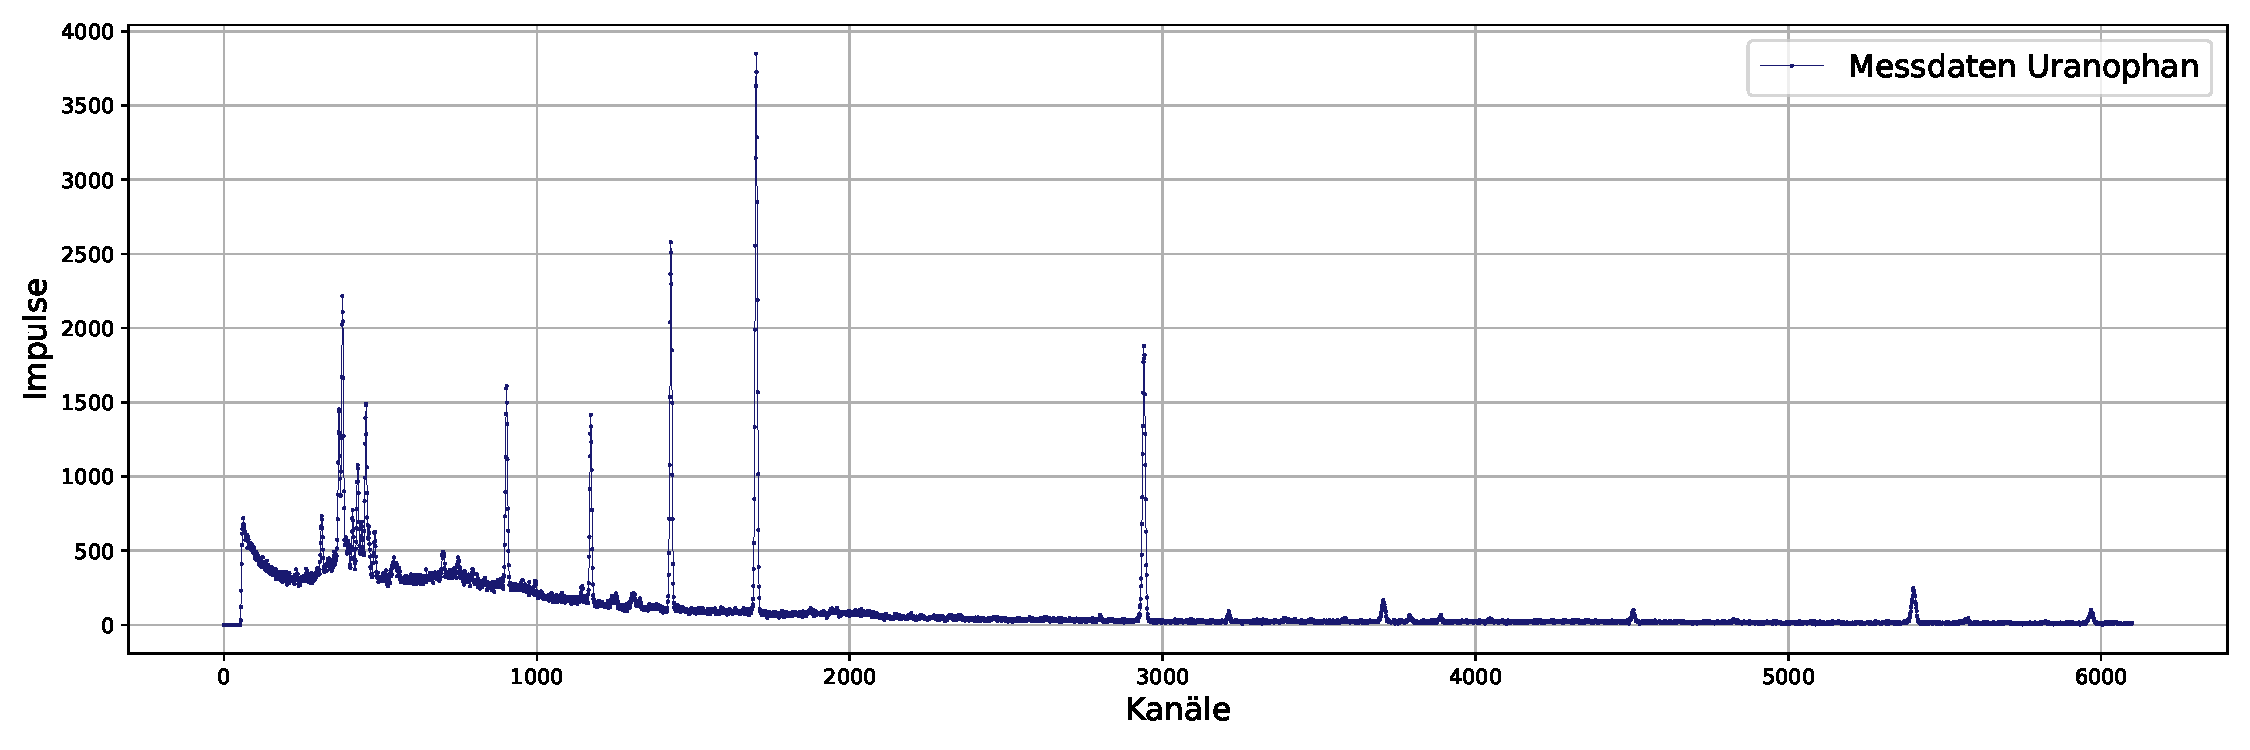
\includegraphics[width = 0.8\textwidth]{plots/uran_channel.pdf}
    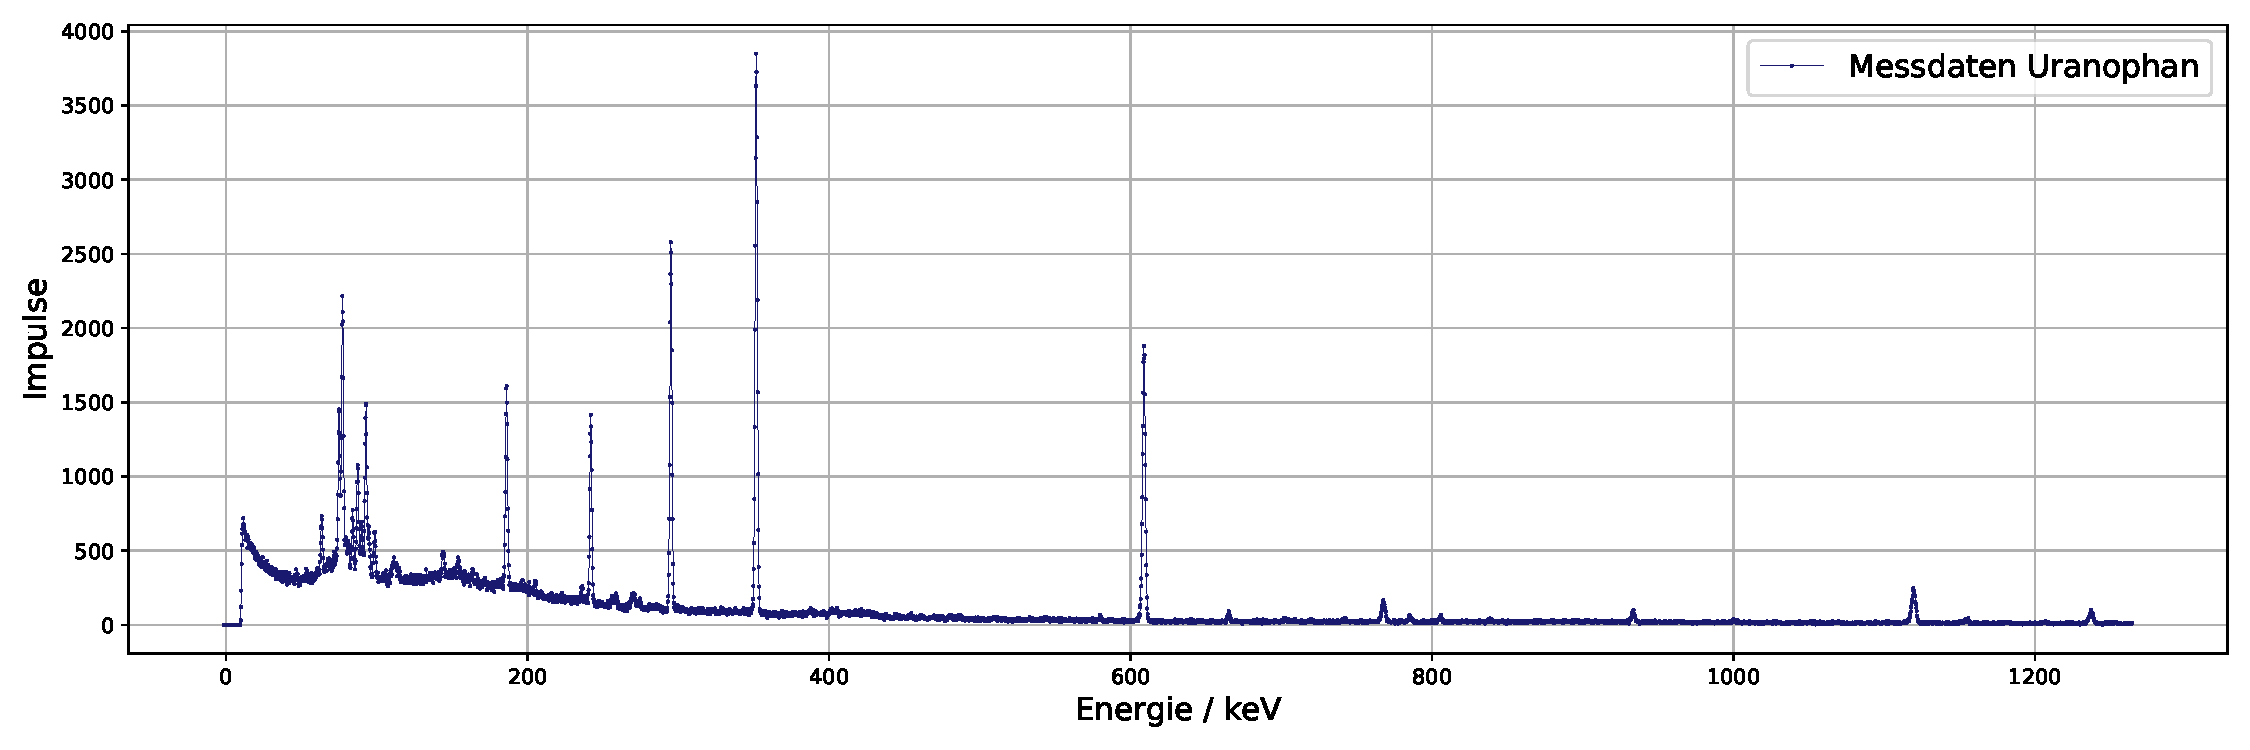
\includegraphics[width = 0.8\textwidth]{plots/uran_energy.pdf}
    \caption{Gammaspektrumaufnahme des Uranophan-Strahlers pro Kanal (oben) und pro Energie in keV (unten). Die Kanäle (bzw. Energie) wurden auf den relevanten Bereich reduziert.}
    \label{fig:Uranophan}
\end{figure}

Es werden alle prominenten Peaks abgelesen und mittels einer durch Scipy\cite{scipy} gefitteten Normalverteilung Position und Linieninhalt bestimmt. Anhand der Uran-Radium-Zerfallskette und der Positionen 
der FEP werden die Nuklide bestimmt und schließlich mittels \autoref{eqn:Aktivitaet} die Aktivität berechnet. Aufgrund von Störfaktoren, werden alle Peaks bis circa $\qty{150}{\kilo\electronvolt}$
nicht berücksichtigt.

\begin{table}
    \centering
    \caption{Peaknummer, Linieninhalt $Z$, Nuklid, Emissionswahrscheinlichkeit $W$, Vollenergienachweiswahrscheinlichkeit $Q$ und Aktivität $A$ pro FEP für das jeweilige Nuklid\cite{Uran_Zerfall}.}
    \label{tab:Barium}
    \begin{tabular}{c c c c c c c}
      \toprule
      $Peak$ & $Z \mathbin{/} \mathrm{Impulse}$ & Nuklid & $W \mathbin{/} \% $ & $E_{\mathrm{FEP}} \mathbin{/} \unit{\kilo\electronvolt}$ & $Q \mathbin{/} \%$ & $A \mathbin{/} \unit{\becquerel}$ \\
      \midrule
      $\qty{1}{}$ & $\qty{16239.63}{}$   & Ra-226 & $\qty{3.56}{}$  & $\qty{186.11 \pm 0.23}{}$ & $\qty{45 \pm 23}{}$ & $\qty{11321.77 \pm 5657.64}{}$ \\
      $\qty{2}{}$ & $\qty{12457.25}{}$   & Pb-214 & $\qty{7.27}{}$  & $\qty{242.03 \pm 0.23}{}$ & $\qty{34 \pm 17}{}$ & $\qty{5612.27 \pm 2867.78}{}$ \\
      $\qty{3}{}$ & $\qty{22204.09}{}$   & Pb-214 & $\qty{18.41}{}$ & $\qty{295.19 \pm 0.23}{}$ & $\qty{28 \pm 14}{}$ & $\qty{4868.62 \pm 2530.08}{}$ \\
      $\qty{4}{}$ & $\qty{34675.62}{}$   & Pb-214 & $\qty{35.6}{}$  & $\qty{351.80 \pm 0.24}{}$ & $\qty{23 \pm 12}{}$ & $\qty{4730.62 \pm 2495.35}{}$ \\
      $\qty{5}{}$ & $\qty{20693.64}{}$   & Bi-214 & $\qty{45.49}{}$ & $\qty{608.99 \pm 0.27}{}$ & $\qty{13 \pm 7}{}$  & $\qty{3937.27 \pm 2175.95}{}$ \\
      $\qty{6}{}$ & $\qty{2531.60}{}$    & Bi-214 & $\qty{4.89}{}$  & $\qty{767.82 \pm 0.30}{}$ & $\qty{10 \pm 6}{}$  & $\qty{5719.02 \pm 3223.19}{}$ \\
      $\qty{7}{}$ & $\qty{1571.51}{}$    & -      & -               & $\qty{933.48 \pm 0.34}{}$ & $\qty{8 \pm 5}{}$   & - \\
      $\qty{8}{}$ & $\qty{4064.16}{}$    & Bi-214 & $\qty{8.94}{}$  & $\qty{1119.50 \pm 0.40}{}$ & $\qty{7 \pm 4}{}$  & $\qty{4478.76 \pm 2605.51}{}$ \\
      $\qty{9}{}$ & $\qty{1693.43}{}$    & -      & -               & $\qty{1237.20 \pm 0.40}{}$ & $\qty{6 \pm 4}{}$  & - \\
      \bottomrule
    \end{tabular}
\end{table}
Somit scheint es sich bei den Gammastrahlern um Radium-226, Blei-214 und Bismut-214 zu handeln. Zwei Peaks konnten keinem Isotop zugeordnet werden.\\
Aus den bestimmten Aktivitäten kann nun mittels der Python Bibliothek Uncertainties\cite{uncertainties} der Mittelwert, sowie Standardabweichung bestimmt werden:
\begin{align}
    A_{\mathrm{Ra}} &= \qty{11321.77 \pm 5657.64}{\becquerel},\\
    A_{\mathrm{Pb}} &= \qty{5070.50 \pm 2630.83}{\becquerel},\\
    A_{\mathrm{Bi}} &= \qty{4711.68 \pm 2667.80}{\becquerel}.
\end{align}
Es ist davon auszugehen, dass es sich bei dem Uran in dem Uranophan um Uran-234 handelt.